\documentclass{beamer}
\usepackage{standalone}

\usepackage{lmodern}% http://ctan.org/pkg/lm
\usepackage{complexity}

\usepackage{tikz}
\usetikzlibrary{arrows,positioning,fit,shapes.multipart,decorations.pathmorphing,overlay-beamer-styles}

\usetheme{Rochester}
\usecolortheme{beaver}

\title{Sequential Games}
\author[M. Dewaskar]{Miheer Dewaskar}
\institute[CMI]{Chennai Mathematical Institute}
\subject{Computer Science}
%
% \AtBeginSection[]
% {
%   \begin{frame}
%     \frametitle{Table of Contents}
%     \tableofcontents[currentsection]
%   \end{frame}
% }

\newenvironment{slide}
{\begin{frame}[environment=slide]
\frametitle{\insertsection}}
{\end{frame}}

\newenvironment{inframe}[2][1]{%
  \edef\inframe@current{\the\value{beamerpauses}}%
  \setcounter{beamerpauses}{#1}%
  \beamer@slideinframe=#2\relax
  \let\beamer@anotherslidetrue=\@empty
  \let\beamer@localanotherslidetrue=\@empty
}{%
  \setcounter{beamerpauses}{\inframe@current}%
}

\newcommand*{\includestandaloneslides}[3][0]{
    \foreach [count=\i] \slide in #2{
        \pgfmathtruncatemacro{\n}{\i + #1}
        \only<\n>{
            \begin{inframe}{\slide}
            \includestandalone{#3}
            \end{inframe}
        }
    }
}

\xdefinecolor{color1}{rgb}{1.0, 0, 0}
\xdefinecolor{color2}{rgb}{0, 0, 1.0}

\begin{document}
  \frame{\titlepage}

  \begin{frame}
    \frametitle{Table of Contents}
    \tableofcontents
  \end{frame}

  \section{Introduction}

  \section{Parity Games}

  \begin{slide}
    \begin{itemize}
      \item Players are called Odd and Even
      \item Additonally, there are  priorities for each vertex
      \[ p : V \mapsto \{1,2\ldots M\} \]
    \end{itemize}
    \begin{block}{Winning Condition}
      Let the play be $\pi = s_0s_1s_2\cdots$
        \[
         %Elaborate%
          P(\pi) = \limsup_i p(s_i)
        \]
    Player Odd wins $\pi$ if $P(\pi)$ is Odd. Otherwise
    %The play is even and%
    Player Even wins.
  \end{block}
\end{slide}

\tikzset{
    p1/.style={circle, draw, thick, minimum size=6mm, inner sep=0},
    p2/.style={rectangle, draw, thick, minimum size=6mm, inner sep=0},
    pre/.style = {<-, semithick, >=stealth', shorten <=1pt},
    post/.style= {->, semithick, >=stealth', shorten >=1pt}
  }
  %\tikzset{
    %invisible/.style={opacity=0},
    %visible on/.style={alt={#1{}{invisible}}},
    %alt/.code args={<#1>#2#3}{%
      %\alt<#1>{\pgfkeysalso{#2}}{\pgfkeysalso{#3}} % \pgfkeysalso doesn't change the path
    %},
  %}

  \begin{slide}
    \framesubtitle{An equivalent finite game}

    \begin{block}{Truncated Game}
      \begin{itemize}
        \item The games stops first time a vertex repeats
        \item The player with the maximum priority in the (unique) loop wins.
      \end{itemize}
    \end{block}

    \pause
    \begin{itemize}
      \item By determinacy of finite games one of the players has a winning strategy in the truncated game.
      \item The same player will also has a winning strategy in the parity game.
    \end{itemize}
\end{slide}

  \begin{slide}
    \framesubtitle{Example}
    \begin{columns}
    \column{.5\textwidth}
    \scalebox{0.65}{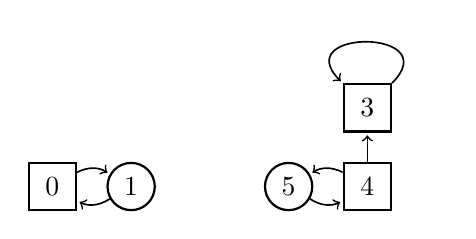
\begin{tikzpicture}
	[podd/.style={circle, draw, thick, minimum size=6mm, inner sep=0},
	peven/.style = {rectangle, draw, thick, minimum size=6mm, inner sep=0},
	pre/.style = {<-, semithick, shorten <=1pt},
	post/.style = {->, shorten >=1pt, semithick}]
	\node (origin) at (0,0) {};
	\node (1) [podd, left of=origin] {1};
	\node (0) [peven, left of=1]  {0}
		edge [post, bend left] (1)
		edge [pre, bend right] (1);
	\node (5) [podd, right of=origin]  {5};
	\node (4) [peven, right of=5]  {4}
		edge [post, bend right] (5)
		edge [pre, bend left] (5);
	\node (3) [peven, above of=4] {3}
		edge [pre] (4)
		edge [loop, post, looseness=4] (3);
\end{tikzpicture}
}
    \column{.5\textwidth}
    \scalebox{0.65}{%!tikz editor 1.0
\documentclass[tikz]{standalone}
\usepackage{tikz}

%!tikz preamble begin
\usepackage{tikz}
\usetikzlibrary{arrows,positioning,fit}

\xdefinecolor{color1}{rgb}{1.0, 0, 0}
\xdefinecolor{color2}{rgb}{0, 0.5, 1.0}
 
\tikzset{
    p1/.style={circle, draw, thick, minimum size=6mm, inner sep=0},
    p2/.style={rectangle, draw, thick, minimum size=5mm, inner sep=0},
    pre/.style = {<-, semithick, >=stealth', shorten <=1pt},
    post/.style= {->, semithick, >=stealth', shorten >=1pt},
  }
%!tikz preamble end

\begin{document}
%!tikz source begin
\begin{tikzpicture}[->, >=stealth', podd/.style=p1, peven/.style=p2, node distance=1cm, level/.style={sibling distance=4cm/#1},shorten >=1pt, emph-p2/.style={very thick,color2,draw}, no-emph/.style={opacity=0}, emph/.style={edge from parent/.append style={emph-p2}}, norm/.style={edge from parent/.append style={black,thin}}, every node/.style={draw=black,thin},
]
		\node[podd] (1) {1} 
			child { 
				node[podd] (l5) {5} 
				child { node[peven] (l6) {6} }
				child {	
					node[peven] (l2) {2} 
					child[emph] { node[peven] (l3) {3}
						child { node[peven] (l6') {6} }
					}
					child[missing] { node {} } 
					}
			}
			child { 
				node[peven] (r2) {2}
				child[missing] { node {} 
				}
				child[emph] { 
					node[peven] (r3) {3}
					child[missing] { node {}
					}
					child[emph] { node [peven] (r6) {6}
						child { node [podd] (r5) {5} 
						}
					}
				}
			};
		\path[dashed] (r2) edge [no-emph, bend left=50] (1)
			  (r3) edge [no-emph, loop, in=180, out=240, looseness=9] (r3)
			  (r5) edge [bend left, out=90] (r2)
			  (r5) edge [bend right, out=-120] (r6)
			  (l6) edge [emph-p2,out=230, in=-180, looseness=2] (l5)
			  (l2) edge [no-emph, out=-60, in=-120, looseness=1] (1)
			  (l6') edge [emph-p2, out=-120, in=-90] (l5);
	  %\begin{scope}[inner sep=2pt, minimum size=1pt]
        %\node (odd-sym) [podd, right=of graph.east , label={right:Odd}, fill=color1] {};
    	%	\node [peven, above=2mm of odd-sym, label={right:Even}, fill=color2] {};
      %\end{scope}
\end{tikzpicture}
%!tikz source end

\end{document}}
    \end{columns}
  \end{slide}

  \begin{slide}
    \framesubtitle{Extracting a winning strategy from the finite game}
    Maintain a stack of vertices as memory -
    \begin{align*}
        M &= \{ u \in V^* \mid \text{no vertex occurs twice in } u \}\\
        m_0 &= v_0
    \end{align*}

    Memory updatation -
    \begin{align*}
        \delta : M \times V \mapsto M \\
        \delta(u_0u_1\cdots u_k, v) &=
            \begin{cases}
                u_0u_1\cdots u_i   &  \text{if } u_i=v\\
                u_0u_1\cdots u_k v & \text{otherwise}
            \end{cases}
    \end{align*}

    Memory based action -
    \[
        \sigma : M \cap V^*V_{even} \mapsto V
    \]
  \end{slide}

  \begin{slide}
    \framesubtitle{Example: extracting a strategy from the finite game}
    \begin{columns}
    \column{.5\textwidth}
    \scalebox{0.65}{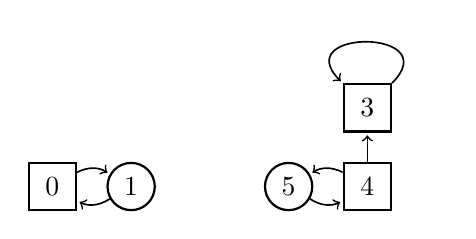
\begin{tikzpicture}
	[podd/.style={circle, draw, thick, minimum size=6mm, inner sep=0},
	peven/.style = {rectangle, draw, thick, minimum size=6mm, inner sep=0},
	pre/.style = {<-, semithick, shorten <=1pt},
	post/.style = {->, shorten >=1pt, semithick}]
	\node (origin) at (0,0) {};
	\node (1) [podd, left of=origin] {1};
	\node (0) [peven, left of=1]  {0}
		edge [post, bend left] (1)
		edge [pre, bend right] (1);
	\node (5) [podd, right of=origin]  {5};
	\node (4) [peven, right of=5]  {4}
		edge [post, bend right] (5)
		edge [pre, bend left] (5);
	\node (3) [peven, above of=4] {3}
		edge [pre] (4)
		edge [loop, post, looseness=4] (3);
\end{tikzpicture}
}
    1 \only<2->{
        \alert<4,9>{5}
        \only<3-4>{6 \only<4->{\alert<4>{5}}}
        \only<6-9>{2 \visible<7->{3} \visible<8->{6} \only<9>{\alert<9>{5}} }
    }
    \column{.5\textwidth}
    \only<-8>{
    \scalebox{0.65}{%!tikz editor 1.0
\documentclass[tikz]{standalone}
\usepackage{tikz}

%!tikz preamble begin
\usepackage{tikz}
\usetikzlibrary{arrows,positioning,fit}

\xdefinecolor{color1}{rgb}{1.0, 0, 0}
\xdefinecolor{color2}{rgb}{0, 0.5, 1.0}
 
\tikzset{
    p1/.style={circle, draw, thick, minimum size=6mm, inner sep=0},
    p2/.style={rectangle, draw, thick, minimum size=5mm, inner sep=0},
    pre/.style = {<-, semithick, >=stealth', shorten <=1pt},
    post/.style= {->, semithick, >=stealth', shorten >=1pt},
  }
%!tikz preamble end

\begin{document}
%!tikz source begin
\begin{tikzpicture}[->, >=stealth', podd/.style=p1, peven/.style=p2, node distance=1cm, level/.style={sibling distance=4cm/#1},shorten >=1pt, emph-p2/.style={very thick,color2,draw}, no-emph/.style={opacity=0}, emph/.style={edge from parent/.append style={emph-p2}}, norm/.style={edge from parent/.append style={black,thin}}, every node/.style={draw=black,thin},
]
		\node[podd] (1) {1} 
			child { 
				node[podd] (l5) {5} 
				child { node[peven] (l6) {6} }
				child {	
					node[peven] (l2) {2} 
					child[emph] { node[peven] (l3) {3}
						child { node[peven] (l6') {6} }
					}
					child[missing] { node {} } 
					}
			}
			child { 
				node[peven] (r2) {2}
				child[missing] { node {} 
				}
				child[emph] { 
					node[peven] (r3) {3}
					child[missing] { node {}
					}
					child[emph] { node [peven] (r6) {6}
						child { node [podd] (r5) {5} 
						}
					}
				}
			};
		\path[dashed] (r2) edge [no-emph, bend left=50] (1)
			  (r3) edge [no-emph, loop, in=180, out=240, looseness=9] (r3)
			  (r5) edge [bend left, out=90] (r2)
			  (r5) edge [bend right, out=-120] (r6)
			  (l6) edge [emph-p2,out=230, in=-180, looseness=2] (l5)
			  (l2) edge [no-emph, out=-60, in=-120, looseness=1] (1)
			  (l6') edge [emph-p2, out=-120, in=-90] (l5);
	  %\begin{scope}[inner sep=2pt, minimum size=1pt]
        %\node (odd-sym) [podd, right=of graph.east , label={right:Odd}, fill=color1] {};
    	%	\node [peven, above=2mm of odd-sym, label={right:Even}, fill=color2] {};
      %\end{scope}
\end{tikzpicture}
%!tikz source end

\end{document}}
}
    \only<9>{
    \begin{itemize}
        \item At each stage a loop with an even priority is eliminated.
        \item Hence the largest priority on the path can't be odd (why?)
    \end{itemize}
    }
    \end{columns}
  \end{slide}

  \begin{slide}
      \framesubtitle{some results}
      We saw that either Odd or Even has a winning strategy - this can be computed using the Truncated game.
      \pause
      \begin{itemize}
          \item Infact, winning player has a positional winning strategy \\
              (this explains why the truncated game works)
          \item A positional strategy $\sigma$ is winning for Odd (Even) iff every reachable cycle in $G_{\sigma}$ has maximum priority odd (even).\\
              (can be checked using SCC decomposition)
          \item Hence the the problem of deciding the winner is in $\NP \cap \coNP$
          \pause
          \item If the number of priorities is bounded, polynomial time solution exist to decide the winner and find the winnnig strategy.
          \item \alert{Open problem} -- is it in $\P$? Only subexponential algorithms known - $\mathcal{O}(n^{\sqrt{n}})$
      \end{itemize}
  \end{slide}

  \section{Mean Payoff Games}

  \begin{slide}
      \framesubtitle{Definition}
      \begin{itemize}
          \item Players are called Max and Min
          \item Edge weights
              \[
                  w : E \mapsto \{-M \ldots, 0, \ldots M\}
              \]
      \end{itemize}
      \begin{block}{Payoffs}
         Let $\pi$ be the run $s_0s_1s_2\ldots$
         \[
             P(\pi) = \liminf_{n} \frac{1}{n}\sum_{i=0}^{n-1} w(s_i,s_{i+1})
         \]
         Player Max wishes to maximize $P(\pi)$ while player Min wishes to minimize it.
      \end{block}
      Player Min pays $P(\pi)$ ``units of money'' to player Max.
  \end{slide}

  \begin{slide}
      \framesubtitle{The equivalent truncated game}
      \begin{block}{Truncated game}
          \begin{itemize}
          \item Stop the first time a vertex repeats
          \item The payoff associated to this play is the average value of the vertices on the (unique) loop formed
          \end{itemize}
      \end{block}

      This is a finite game, hence it has a minimax value i.e -
      \begin{itemize}
          \item There is a $v \in \mathbb{Q}$
          \item Max has a strategy $\sigma^*$ which ensures that the first loop formed has average value $\geq v$.
          \item Min has a strategy $\tau^*$ which ensures that the first loop formed has avergae value $\leq v$.
      \end{itemize}
  \end{slide}

  \begin{slide}
      \framesubtitle{Extending the strategy to mean payoff games}
      \begin{itemize}
          \item Extend $\sigma^*$, $\tau^*$ to the infinite duration game similar to parity games.
          \item The extension of $\sigma^*$  ensures that every eliminated loop has average value $\geq v$. Hence the $\liminf$ of averages on the entire path will be $\geq v$.
          \item Similarly, the extension of $\tau^*$ ensures that every eliminated loop has average value $\leq v$. Hence the $\limsup$ of averages on the entire path will be $\leq v$.
      \end{itemize}
      \pause
      Hence the mean payoff game has the value $v$! \\
      Extensions of $\sigma^*$ and $\tau^*$ are the optimal strategies.
  \end{slide}

  \begin{slide}
      \framesubtitle{Some results on mean payoff games}
      \begin{itemize}
        \item Each player has positional optimal strategies.
        \item The decision problem - \alert{is the value $\geq 0$?} is in $\NP \cap \coNP$ \\
            (Via reduction to stochastic/mean payoff games)
        \item Pseudo polynomial algorithm (polynomial in the unary representation of the weights) by looking at the sum game.
      \end{itemize}

      \begin{block}{Similarity to Parity Game?}
          Let $w(u,v) = (-|E|)^{p(u)}$\\
          A simple cycle has average value $\geq 0$ iff the max priority in the cycle is even.\\ \pause
          Hence value of the truncated game $v \geq 0$ iff player Even has a winning trategy in the truncated game.
      \end{block}

      Reduces parity to mean payoff.
  \end{slide}
  %
  % \section{References}
  %
  %   \begin{thebibliography}{1}
  %     \bibitem{up} Jurdziński, Marcin. “Deciding the Winner in Parity Games Is in UP∩ Co-UP.” Information Processing Letters 64, no. 3 (1998): 119–24.
  %     \bibitem{subexp} Jurdzinski, Marcin, Mike Paterson, and Uri Zwick. “A Deterministic Subexponential Algorithm for Solving Parity Games.” SIAM Journal on Computing 38, no. 4 (2008): 1519–32.
  %   \end{thebibliography}
  \section{Simple Stochastic Games}
\end{document}
